\section{Г-функция Эйлера}

\begin{definition}
    $\Gamma(p) = \int_0^{+\infty }x^{p-1}e^{-x}dx$

    $p >0$
\end{definition}

\begin{property}
    \[\Gamma(p+1) = p\Gamma(p)\quad \forall p >0\] -- формула приведения

    \[\Gamma(p) = \frac{\Gamma(p+1)}{p}\] -- определение для $\Gamma$ в $\R\setminus \left( \Z_- \right) $

    \begin{align*}
    \Gamma(1) &= 1\quad \Gamma(p + 1) = p!\\
    \Gamma(\frac{1}{2}) &= \frac{e^{-x}}{\sqrt{x}}dx = 2\int_0^{+\infty }e^{-t^2}dt = 2 \cdot \frac{\sqrt{\pi}}{2} = \sqrt{\pi}\\
    \Gamma(\frac{3}{2}) &= \frac{1}{2} \Gamma(\frac{1}{2}) = \frac{\sqrt{\pi} }{2}\\
    \Gamma(\frac{5}{2}) &= \frac{3\sqrt{\pi} }{4}\\
    \Gamma(\frac{2n+1}{2}) &= \frac{(2n-1)!!}{2^n} \sqrt{\pi} \text{(по индукции)}\\
    .\end{align*}
\end{property}

\begin{note}[Дифиренцирование $\Gamma$--функции]
    \[
    \Gamma^{(k)}(p) = \int_0^{+\infty } \underbrace{x^{p-1}e^{-x} \left( \ln x \right) ^k}_{f_k(x, p)} dx
    .\]

    $\frac{\partial f_k(x, p)}{\partial p} = f_{k+1}(x, p)$
\end{note}

\begin{note}
    Локальное условие Лебега $\forall p_0$?

    \[
    \exists V_{p_0}: \exists \Phi(x) \in \mathcal L \left( \left( 0, +\infty  \right): \left| f_k(x, p) \right| \leqslant \Phi(x)  \right)
    .\]

    \begin{align*}
        x^{p-1} & \leqslant x^{2p_0-1} + x^{\frac{p_0}{2}-1} \\
        \Phi(x) &= \left( x^{2p_0-1} + x^{\frac{p_0}{2}-1} \right)e^{-x}\left| \ln x \right| ^k.
    \end{align*}
    $\Phi$ -- мажоранта для $f_l(x, p) \forall p\in V_{p_0}$

    \begin{align*}
        \int_0^{+\infty }x^{p-1}e^{-x} \left| \ln x \right| ^kdx &< +\infty \\
        x^{p-1}|\ln x|^k = o(e^{\frac{x}{2}})\quad  x \to+\infty \\
        x^{p-1}e^{-x}\left| \ln x \right| ^k &\sim x^{p-1}\left| \ln x \right| ^k = o(x^{p-1-\alpha})\\
        &|\ln x |^k = o(x^{-\alpha}),~~ \alpha > 0\\
        x \to 0^{+}~~~ p -\alpha > 0.
        \end{align*}

    Получается, что $\Gamma$ -- класса $C^{\infty }$ там, где она определена. $\Gamma \in C^{\infty }\left( \R\setminus \Z _-  \right) $
\end{note}

\paragraph{Геометрические характеристики $\gamma$--функции и элементарные факты}

\begin{property}[Геометрические свойства]
\begin{enumerate}
    \item $\gamma(p)$ строго выпукла на любом отрезке, лежащем в её области определения
    \item На $(0, +\infty )$ $\Gamma(p)$ имеет единственный экстремум в точке $c\in (1, 2)$
    \item $p\to 0\quad \Gamma(p) \sim \frac{1}{p}$
\end{enumerate}
\end{property}
\begin{proof}
    $\Gamma^{(2)}_{p^2}(p) = \int_0^{+\infty }x^{p-1}e^{-x}ln^2x dx >0 \implies 1$

    $\Gamma(1) = 0! =1 = 1! = \Gamma(2) \implies $ по теореме Роля $\exists c\in (1, 2):\quad \p \Gamma(c) = 0$. $c$ -- точка минимума

    $\p \Gamma(p)\neq 0$ при $p\neq c, p>0$
\end{proof}

\begin{figure}
    \centering
    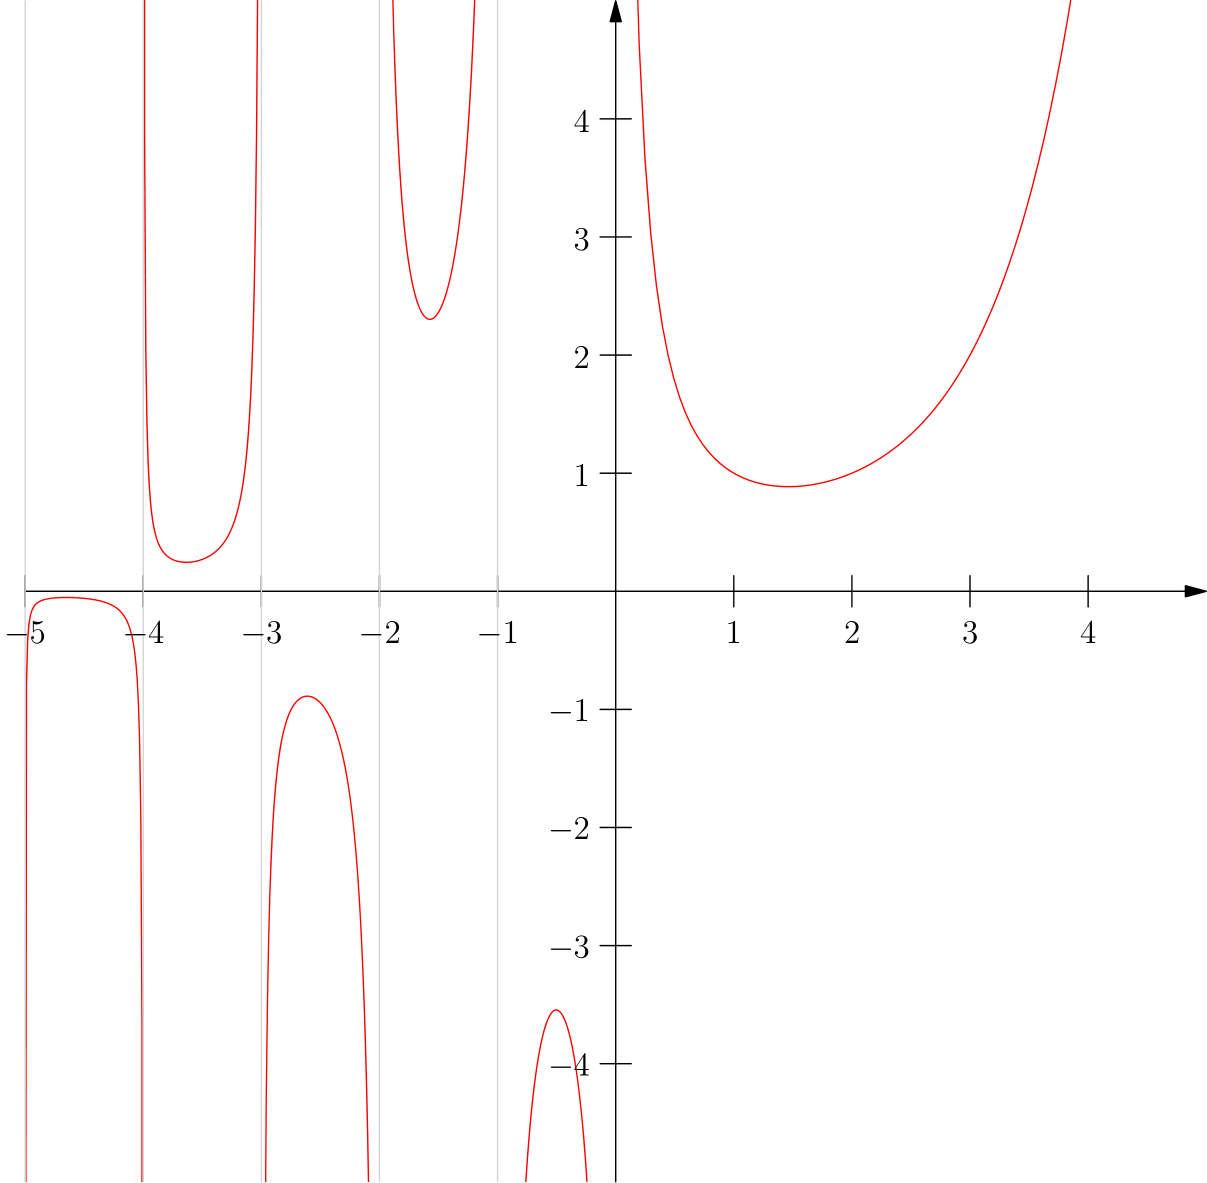
\includegraphics[width=0.5\textwidth]{./figures/gamma_function.png}
    \caption{gamma-function}
    \label{fig:gamma-function}
\end{figure}

% %\begin{figure}
%     %\centering
%     %\begin{tikzpicture}
%         %\begin{axis}[
%             %xmin = -4.9, xmax = 5.1,
%             %%ymin = -3.5, ymax = 3.5,
%             %restrict y to domain=-6:6,
%             %axis lines = middle,
%             %axis line style={-latex},
%             %xlabel={$x$},
%             %ylabel={$y$},
%             %%enlarge x limits={upper={val=0.2}},
%             %enlarge y limits=0.05,
%             %x label style={at={(ticklabel* cs:1.00)}, inner sep=5pt, anchor=north},
%             %y label style={at={(ticklabel* cs:1.00)}, inner sep=2pt, anchor=south east},
%             %]
%             %
%             %\addplot[color=red, samples=222, smooth,
%             %domain = 0:5] gnuplot{gamma(x)};
%             %
%             %\foreach[evaluate={\N=\n-1}] \n in {0,...,-5}{%
%             %\addplot[color=red, samples=555, smooth,
%             %domain = \n:\N] gnuplot{gamma(x)};
%             %%
%             %\addplot [domain=-6:6, samples=2, densely dashed, thin] (\N, x);
%             %}%
%             %\end{axis}
%     %\end{tikzpicture}
%     %\caption{Гамма-функция}
%     %\label{Гамма-функция}
% %\end{figure}

% %\psset{unit=1.25cm}
% %\begin{pspicture*}(-4.8,-4.8)(4.8,4.8)
% %\psaxes[ticksize=2pt -2pt]{->}(0,0)(-4.8,-4.8)(4.8,4.8)[$ x $, -120][$ y $, -140]
% %\psset{linecolor=Tomato3,linewidth=1.2pt,plotpoints=100,algebraic}
% %\psplot{-4.995}{-4.005}{GAMMA(x)}
% %\psplot{-3.995}{-3.01}{GAMMA(x)}
% %\psplot{-2.99}{-2.05}{GAMMA(x)}
% %\psplot{-1.95}{-1.05}{GAMMA(x)}
% %\psplot{-0.9}{-0.1}{GAMMA(x)}
% %\psplot{.1}{5.8}{GAMMA(x)}
% %\psset{linewidth = 0.6pt, linecolor = LightSteelBlue3}
% %\multido{\i=-4+1}{4}{\psline(\i, -5.8)(\i, 5.8)}
% %\end{pspicture*}

\begin{note} Аналог формулы стрилинга.
     При $p \to \infty $  верно, что $\Gamma (p) = \sqrt {2 \pi p} \left( \dfrac{p}{e} \right) ^p e^{\frac{\Theta}{12}}$, где $\Theta \in (0, 1)$.
\end{note}

\section{Бета-функция}

\begin{definition}
    $B(p, q) = \int_0^1 x^{p-1}(1-x)^{q-1}dx$

    $B(p, q) = B(q, p) \forall p, q > 0$

    $B(p, q) = \frac{\Gamma(p)\Gamma(q)}{\Gamma(p + q)}$
\end{definition}

\begin{theorem}
    [формула Эйлера-Гаусса]

    \[
    \Gamma(p) = \lim_{k \to \infty} \frac{l^p \cdot k!}{p(p-1) \ldots (p+k)} \quad \forall p\in \R\setminus \Z _-
    .\]
\end{theorem}

\begin{proof}
    \begin{align*}
        \Gamma(p ) &=\int_0^{+\infty} x ^{p-1} e ^{-x } dx = \Bigg| t = e^{-x}, x = -\ln t, dx = - \dfrac{dt}{t} \Bigg| \int _0^1 (-\ln t)^{p-1} t  \left(- \dfrac{dt}t\right) = \int_{0}^1 (-\ln t)^{p-1)}\\
        &= \int_0^1 \left( \lim_{k\to\infty} \underbrace{k (1 - t^{1/k})}_{g(k)}\right)^{p-1} dt ==\\ %
        \p g (k) &= (1 - t^{1/k}) + k (- t^{1/k})\cdot (\ln t) \cdot  \left( + \dfrac{1}{k^2} \right)\\
        &= t^{\frac{1}{k}}\left( t^{- \frac{1}{k}}  - 1 + \frac{\ln t}{k}\right)  \\
        &= \begin{cases}
            f\uparrow&, \text{ если } p\geqslant 1 \implies \text{Применим теорему Леви}\\
            f\downarrow&, \text{ если } p\in (0,1) \implies g(k) \leqslant g(1)\\
        \end{cases} \\
        &== \lim_{k \to \infty} \int_0^1 \left( k(1 - t^{\frac{1}{k}}) \right)^{p-1}dt  = \lim_{k \to \infty} k^{p-1} \int_0^1 s^{p-1} (-k)(1-s)^{k-1}ds = \lim_{k \to \infty} k^p B(p, k) \\
        &= \lim_{k \to \infty} k^p \frac{\Gamma(p)\Gamma(k)}{\Gamma(p+k)} = \lim_{k \to \infty} k^p \cdot (k-1)! \frac{\Gamma(p)}{(p+k-1)(p+k-2)\ldots p \Gamma(p)}\\
        &= \frac{k^pk!}{p(p+1)\ldots (p+k)} \cdot \underbrace{\frac{p+k}{k}}_{\to 1}.
    \end{align*}

    Для $ p<0$ по индукции по $m\quad p \in \left( -(m+1) , -m\right)  $

    Если формула верна для $p+1$, то
    \begin{align*}
    \Gamma(p) &= \frac{\Gamma(p+1)}{p}  = \frac{1}{p} \lim_{k \to \infty} \frac{k^{p+1}\cdot k!}{(p+1)(p+2) \ldots (p+k+1)}\\
    &=\lim_{k \to \infty} \frac{k^p\cdot k!}{p(p+1) \ldots (p + k)} \cdot \underbrace{\frac{k}{p+k+1}}_{\to 1}
    .\end{align*}
\end{proof}

\begin{lemma}
Пусть $a \in \R$, $f(x) \in C([a, +\infty))$ и $f$ ограничена на $([a, +\infty))$~:~~$\int_a^{+\infty } f(x) dx$ сходится.
Тогда \[I(y) = \int_a^{+\infty }e^{-xy}f(x)dx \in C([0, +\infty )).\]
\end{lemma}
\begin{proof}
    $A \in [a, +\infty)$

    \begin{align*}
        \int_A^{+\infty }e^{-xy} f(x) dx &= \Bigg| F(x) = \int_A^x f(t)dt \Bigg|  = (F(x) - F(A))\cdot e^{-xy}\mid_A^{+\infty } + \int_A^{+\infty } ye^{-xy} ( F(x) - F(A) ) dx\\
        &= \Bigg| \exists \lim_{x \to \infty} F(x) \left( = \int_A^{+\infty } f(t) dt \right).
    \end{align*}

    Для $\varepsilon >0 \exists A: \left| \int_X^{+\infty }f(t)dt \right| < \frac{\varepsilon}{3}\quad \forall x \geqslant A $

    Для $x \geqslant A\quad \left| F(x) - FA(A) \right|  = \left| \int_X^{+\infty }f(t)dt \right|< \frac{\varepsilon}{3} $

    \begin{align*}
    \left| I_A(y) \right| &\leqslant \int_A^{+\infty }ye^{-xy}\left| F(x) - F(A) \right|dx \\
    &< \frac{\varepsilon}{3}\int_0^{+\infty } ye^{-xy}dx = \frac{\varepsilon}{3}\\
    I(y) &= \overbrace{\int_a^Ae^{-xy}f(x)dx}^{J_A(y)} + I_A(y)\\
    I(y) - I(y_0) &= J(y) - J(y_0) + \overbrace{I_A(y) - I_A(y_0)}^{< \frac{\varepsilon}{3}}
    .\end{align*}

    $J(y) - J(y_0) \to 0$ при $y \to y_0$ (условие непрерывности собственных интегралов).
    \[\exists V(y_0):\quad \forall y\in V(y_0)\, \left| J(y) - J(y_0) \right|< \frac{\varepsilon}{3}. \]
\end{proof}

\begin{corollary}
    \[
    \int_a^{+\infty }f(x)dx = \int_a^{+\infty }\lim_{y \to 0} e^{-xy}f(x)dx.\]
\end{corollary}

\begin{example}
    [Одно из значений интегрального синуса]
    \begin{align*}
        \int_{0}^{+\infty} \dfrac{\sin x} { x}&\\
        I(y) &= \int_0^\infty \underbrace{e^{-xy } \dfrac{\sin x}{x}}_{f(x,y)} dx\\
        \frac{\partial f}{\partial x} &= -e^{-xy}\sin x\\
        y_0 > 0\quad V_{y_0} &= \left( \frac{y_0}{2}, 2y_0 \right) \implies \left| \frac{\partial f}{\partial y} \right| \leqslant e^{-\frac{xy_0}{2}}\\
        \implies \forall y_0& \p I(y) = -\int_0^{+\infty }e^{-xy}\sin x dx\ldots\\
        I(y) &= \int_0^{+\infty} e^{-xy} d cos x = cos x \cdot e^{-xy} \mid_0^{+\infty} + y \int_{0}^{+\infty} \p(\sin x) e^{-xy} dx\\
        &= -1  +  y\left( \sin x e^{-xy} \mid_0^{+\infty} +y \int_{0}^{+\infty} \sin x e ^{-xy} dx \right) = -1 + y^2 \left(-I(y) \right)\\
        \implies& I(y) \cdot(1 + y^2) = -1.\\
        \p I(y) &= I(y) = \left( - \dfrac{1}{1 + y^2}\right) \implies I(y) = C - \int \dfrac{dy}{1+y^2} = C - \arctg y \\
        y\to +\infty, y \geqslant 1& \bigg| e^{-xy} \dfrac{\sin x } {x} \bigg| \leqslant e^{-x}\text{~--- суммируемая мажоранта.}\\
        C - \dfrac{\pi}{2} &= \lim_{y\to \infty} e^{-xy} \dfrac{\sin x} {x} dx = 0 \implies C = \dfrac{\pi}2\\
        I(y)& = \dfrac{\pi}2 - \arctg y \forall y > 0.
    \end{align*}
    Но по лемме $I(y)$ неотрицательная в точке $y = 0$.
    \[ I(0) = \lim_{y \to 0} I(y) = \lim_{y \to 0} \left( \dfrac{\pi}2 - \arctg y \right) =\dfrac{\pi}2 \implies \int_0^{+\infty } \dfrac{\sin  x}x dx = \dfrac{\pi}2. \]
\end{example} %ура, ноль ошибок

\paragraph{Дифференцирование интеграла по параметру в случае переменных пределов интегрирования.}

\[ I(y) = \int_{\alpha(y)}^{\beta(y)} f(x, y) dx;~~~ f \in C \left( [a, b] (x \ni) \times [c, d]  (\ni y)\right),~~~
\alpha(y), \beta(y) : [c, d] \to [a, b] \text{ дифф.}
\]


\begin{figure}
    \centering
    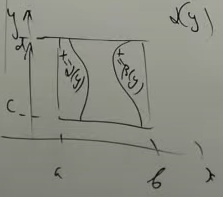
\includegraphics[width=0.3\textwidth]{./img/intergal-with-parametric-bounds.png}
    \caption{Инетграл с переменными пределами}
\end{figure}

\begin{theorem}
    [Правило Лейбница]
Тогда $I(y)$ дифференцируемо на $[c, d]$ и
\[
    I(y) = \int_{\alpha(y)}^{\beta(y)}\p f_y(x, y)dx + f(\beta(y), y)\cdot \p \beta(y) - f\left( \alpha(y), y \right) \cdot \p\alpha(y)
.\]
\end{theorem}
\begin{proof}
    \begin{align*}
        \Phi(x, y) &= \int_a^x f(t, y)dt \\
        \frac{\partial \Phi}{\partial x} &= f(x, y) \text{ непрерывна в }Q\\
        \frac{\partial \Phi}{\partial y} &= \lim_{\Delta \to y} \frac{1}{\Delta y} \left( \int_a^x f(t, y + \Delta y)dt - \int_a^x f(t,y )dt \right)\\
        &= \int_a^x \p f_y(t, y)dt \\
        \frac{\partial \Phi}{\partial y}(x_1, y_1) - \frac{\partial \Phi}{\partial y}(x, y) = \int_a^x \p f_y(t, y_1)dx  + \left( \int_a^x \p f_y(t, y)dx - \int_a^x \p f_y(t, y)dx \right)  - \int_a^x \p f_y(t, y)dx
    .\end{align*}

    Таким образом $\Phi(x, y)$ дифферецируема на $Q$
    \begin{align*}
        I(y) &= \Phi(\beta(y), y) - \Phi(\alpha(y), y) \\
        \p I(y) = \p Phi_x(\beta(y), y)\cdot \p \beta(y) + \p \Phi_y(\beta(y), y) - \p \Phi_x(\alpha(y), y)\cdot \p \alpha(y) - \p\Phi_y(\alpha(y), y).
    \end{align*}
\end{proof}

\begin{example}
    \[I(p) = \int_{p^2}^{p^3} \dfrac{x^2+ 2p }{\ln^2 |x| + 1} dx \]

    $\forall p \neq 0,\quad [a,b] = [p-\delta, p + \delta]\quad [c,d]$
    \[ \p I(p ) = \int_{p^2}^{p^3} \dfrac{2}{\ln^2 |x| + 1}  dx + \dfrac{p^6 + 2p}{\ln^2 |p^3 | + 1} \cdot 3 p^2 - \dfrac{p^4 + 2p}{\ln^2 |p^2 | + 1} \cdot 2p.\]
\end{example}

\section{Интегрирование на многообразиях}

\begin{definition}
    $\gamma: [a,b] \to \R$ кусочно-гладкое, простой путь (биекция) или заскнутый простой (едиснтвенная точка самопересечния -- концы).

    Пусть $\Gamma = \gamma ([a, b])$~--- носитель нашего пути\dots

    $\mathscr{B} = \{ B~\mid~ \gamma^{-1} (B) \in \mathscr{A}$.

    $ds = \nu(B) = \int_{\gamma^{-1}(B)} \|\p \gamma\|(t)dt$.

    $f~:~ \Gamma \to \R(\C)$. $\int_B f ds = \int_{\gamma^{-1} (B) } f (\gamma(t)) \cdot \| \p \gamma (t) \|$.

    Интеграл не зависит от выбора параметризации. Также не зависит от ориентации кривой.
\end{definition}

\begin{example}
    $\int_C x^2sd\qquad C: \begin{cases}
        x^2+y^2+z^2 = R^2\\
         x+y+z = 0\\
    \end{cases}$

    \begin{align*}
        I = \int_C x^2ds = \int_C y^2ds = \int_C z^2ds
        \implies I = \dfrac{1}{3 } \int_C \underbrace{x^2 + y^2 + z^2}_{= R^2} ds = \dfrac{R^2} {3} \int_C ds = \dfrac{R^2} {3} \cdot 2\pi R.
        .\end{align*}
\end{example}

%% нижняя строка, которую можно двигать